
\documentclass{article}
\usepackage[c]{documentation}
%Use Build -> Latex -> DVI.
%ffslides does not accept PDF without extra step.
%Command: dvips -> gv lab &

%Redirecting compiling messages to a log file:
%latex lab > log && tail log
\usepackage{graphicx}
\begin{document}
\title{Dictionary Program}
\author{Omid Niroumandzadeh}
\section{Dictionary Program}
\subsection{Header File: "dictionary.h"}
Our "dictionary.h" file includes the structure "entry". The 
string variables "english" and "spanish" will be used
as placeholders to store the parced data from our
"dict.dat" dictionary file.
\inputsourcecode{dictionary.h}
\clearpage
\subsection{Reading the "dict.dat" File: "readFile.cpp"}
In the "readFile" function, we pass our vector "store" as a 
parameter (through direct reference). We create the following: 
variable "a" of type "entry" (our structure); two strings ("en" and "s")
to store and pass on value to the structure variables; our 
variable "ifs" of data-type "ifstream" which passes in our
"dict.dat" file.

Our control structure (if-statement) opens "ifs" as the condition. 
We then use a while-loop inside the control structure to parse
the file, checking for tab-spaces to separate the data. The parsed
data is passed on to our variables "en" and "s", which is set equal
to the variables inside our structure "a".

The structure is then pushed into our vector "store", allowing us
to close the "dict.dat" file.
\inputsourcecode{readFile.cpp}
\clearpage
\subsection{Taking User Input: "userInput.cpp"}
Our "userinput.cpp" file will be displaying a prompt to take user input.
The vector "store" is passed in by reference in the function's
parameter.

We create a while-loop to prompt the user using a boolean
conditional. A user input of "q" or "Q" will end the loop
and end the program.

Another while-loop checks for correct user input. For example,
an input of integers would repeat the prompt and clear the
previous input.

A successful user input is then taken and compared to every position
inside the vector. Because our vector is of the data-type "entry" 
(declared in "lab.h"), the user's input is stored as the variable 
"english".  
\inputsourcecode{userInput.cpp}
\clearpage
\subsection{Main File: "main.cpp"}
The main function is used to bring all of our different files
together. Inside, we declare our vector "store" as a local variable,
and we pass it on as a parameter into the functions "readFile" and
"userInput".
\inputsourcecode{dictionary.cpp}
\clearpage
\subsection{Screenshots}
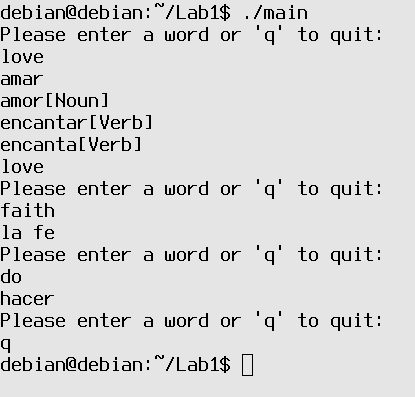
\includegraphics[scale=.8]{test1.png}
\end{document}
